\chapter{导数与微分}

本章主要讨论导数和微分的概念以及它们的计算方法,
至于导数的应用,将在第三章讨论。

\section{导数概念}

    \subsection{引例}

    为了说明微分学的基本概念--导数,我们先讨论两个问题:
    速度问题和切线问题。
    这两个问题在历史上都与导数概念的形成有密切关系。
        
    \subsubsection{直线运动的速度}

    设某点沿直线运动。
    在直线上引入原点和单位点(即表示实数1的点), 使直线成为数轴。
    此外,再取定一个时刻作为测量时间的零点。
    设动点于时刻$t$在直线上位置的坐标为$s$(简称位置$s$).
    这样,该点的运动完全由某个函数

    \[s=f(t)\]

    所确定。
    此函数对运动过程中所出现的$t$值有定义,称为位置函数。
    在最简单的情形,该动点所经过的路程与所花的时间成正比。
    就是说,无论取哪一段时间间隔,比值

    \begin{equation} 
        \frac{\text{经过的路程}}{\text{所花的时间}}
        \label{eq:ratio1}
    \end{equation} 

    总是相同的。
    这个比值就称为该动点的速度,并说该点作匀速运动。
    如果运动不是匀速的,那么在运动的不同时间间隔内,
    比值\eqref{eq:ratio1}会有不同的值。
    这样,把比值\eqref{eq:ratio1}笼统地称为该动点的速度就不合适了,
    而需要按不同时刻来考虑。
    那么,这种非匀速运动的动点在某一时刻(设为$t_0$)的速度应
    如何理解,又该如何求得呢?

    首先取从时刻$t_0$到$t$这样一个时间间隔,在这段时间内,
    动点从位置$s_0=f(t_0)$移到到$s=f(t)$。
    这时由\eqref{eq:ratio1}式算得的比值

    \begin{equation}
        \frac{s-s_0}{t-t_0}=\frac{f(t)-f(t_0)}{t-t_0}
        \label{eq:ratio2}
    \end{equation}

    可认为是动点在上述时间间隔内的平均速度。
    如果时间间隔选得较短,
    这个比值\eqref{eq:ratio2}在实践中也可用来说明动点
    在时刻$t_0$的速度。
    但对于动点在时刻$t_0$的速度的精确概念来说,
    这样做是不够的。
    更确切的说法是:
        令$t\to t_0$,取\eqref{eq:ratio2}式的极限,
        如果这个极限存在,设为$v$,即
    
        \[v=\lim_{t\to t_0} \frac{f(t)-f(t_0)}{t-t_0}\]

    这时就把这个极限值$v$称为动点在时刻$t_0$的(瞬时)速度。

    \subsubsection{切线问题}

    圆的切线可定义为"与曲线只有一个交点的直线", 但是对于其他曲线,
    用这样的定义就不一定合适。
    切线的定义如下:

    设有曲线$C$及$C$上的一点$M$(图\ref{fig:2o1}),
    在点$M$外另取一点$N$,作割线$MN$.
    当点$N$沿曲线$C$趋于点$M$时,
    如果割线$MN$绕点$M$旋转而趋于极限位置$MT$,
    直线$MT$就称为曲线$C$在点$M$处的切线.
    这里极限位置的含义是:只要弦长$|MN|$趋于零,

    \begin{figure}[htp]
        \centering
        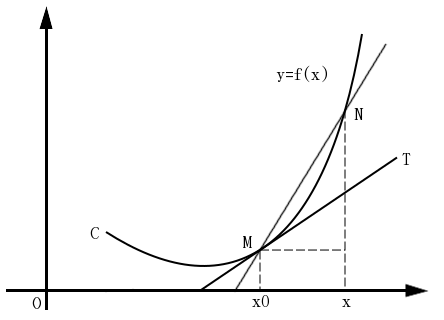
\includegraphics[scale=0.5]{c2/fig_2-2.png}
        \caption{}
        \label{fig:2o2}
    \end{figure}

